\subsection{Sistema de Medición}

Con lo tratado en la sección del sistema de control del capítulo \ref{analisis}, se estableció que para realizar un adecuado control de la plataforma, se debe tomar información de cuatro variables de estado del sistema: la tensión y corriente de la pila de combustible ($v_{FC}$ e $i_{FC}$) y la tensión y corriente de salida ($v_o$ e $i_o$). En esta sección se va a tratar el diseño del sistema de medición de datos de la figura \ref{diag_medicion}, que incluye el sensado de los parámetros del convertidor, el acondicionamiento de las señales, y la transmisión de las mismas al sistema de control.\\

\begin{figure}[h]
    \centering
    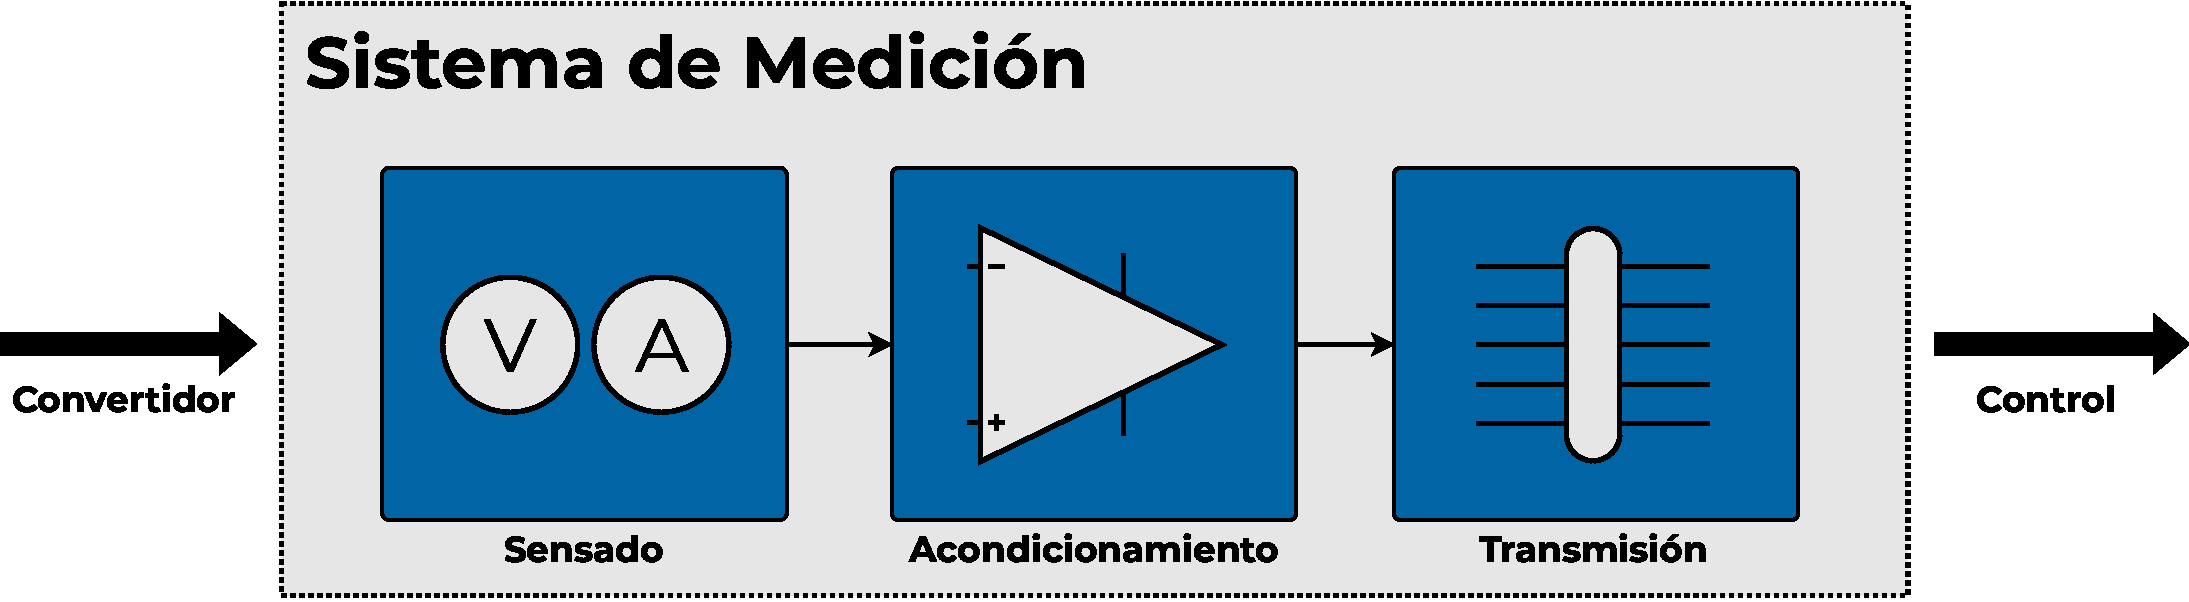
\includegraphics[scale=0.4]{Imagenes/Sistema Medicion.pdf}
    \caption{Sistema de medición de la plataforma, con las tres etapas que lo conforman.}
    \label{diag_medicion}
\end{figure}

Este sistema comienza con la adquisición de los parámetros de interés provenientes del convertidor, tarea llevada a cabo por los sensores de tensión y corriente que conforman la {\Medium etapa de sensado}. Sin embargo, estos datos obtenidos no se presentan en una forma que nuestro sistema de control sea capaz de procesar, por lo que se necesita la siguiente etapa del sistema, la {\Medium etapa de acondicionamiento}, que se encarga de adecuar los datos obtenidos por los sensores para que puedan ser utilizados por el controlador. Finalmente, necesitamos una forma de llevar estos datos desde el sistema de medición hasta el controlador, función que es llevada a cabo por el último bloque de la figura, la {\Medium etapa de transmisión}.\\

Vamos a tratar el diseño de este sistema en el orden que se observa en la figura, por lo que se comenzará por la etapa de sensado o adquisición de datos.\\

\subsubsection{Etapa de Sensado}

En este sistema, los únicos parámetros a medir son tensiones y corrientes, tanto de la pila de combustible a la entrada como de la carga variable a la salida. Previamente a la seleccion de los sensores a utilizar, vamos a realizar una breve categorización y explicación de los métodos de sensado disponibles para ambos parámetros, comenzando por las tensiones.\\

\paragraph{Tecnologías de Sensado de Tensión}

Este es el más simple de los dos casos, ya que los sistemas de control ya trabajan con señales expresadas en tensiones, por lo que no es requerido ningún tipo de transductor, únicamente una adaptación de niveles que es llevada a cabo por la etapa de acondicionamiento. Por esta razón, lo único necesario en este caso es la obtención directa de la tensión buscada, siempre minimizando la perturbación que esta medición introduce al sistema.\\

\paragraph{Tecnologías de Sensado de Corriente}

A diferencia del caso de las tensiones, para poder obtener una medición de corriente se debe realizar algún tipo de transducción que transforme la información de corriente en valores de tensión que puedan ser utilizados por el sistema de control. Existen múltiples tecnologías de sensado y transucción de corriente fundamentalmente distintas, cada una con sus propias características, ventajas y desventajas. Vamos a dedicar algunos párrafos a su clasificación y descripción.\\

\subparagraph{Resistencia Shunt}

Es el método conceptualmente más sencillo de todos, y consiste en interponer al camino de la corriente un resistor \textit{shunt} $R_S$, es decir una resistencia de muy bajo valor (generalmente en las decenas y unidades de \unit{\milli\ohm}), y luego medir la caída de tensión en el mismo. Esta corriente se encuentra directamente relacionada con la tensión mediante la Ley de Ohm, que luego de reordenar resulta:

\begin{equation}\label{ec_shunt}
    I=\frac{1}{R_S}V_S
\end{equation}

Entonces, con este método se obtiene una relación {\Medium perfectamente lineal} entre entre la tensión medida directamente y la corriente que se quiere obtener, siendo el inverso del valor del resistor (o su conductancia) la constante de proporcionalidad. Al tener la Ley de Ohm como su principio de funcionamiento, este método es capaz de medir todo tipo de corrientes, tanto continua (CC) como alterna (CA). Además, al necesitar únicamente una resistor, es {\Medium sumamente sencillo} de implementar.\\

Sin embargo, al estar circulando toda la corriente a través del resistor, se genera una {\Medium pérdida de energía significativa}, ya que la potencia disipada depende del cuadrado de la corriente. Si tomamos la plataforma como ejemplo, donde la corriente de pila $i_{FC}$ en el primario puede llegar a un máximo de \SI[]{10}[]{\ampere}, una resistencia shunt de \SI[]{50}[]{\milli\ohm} puede llegar a disipar una potencia de \SI[]{5}[]{\watt}. Por esta razón, este método no es factible para mediciones de grandes corrientes.\\

La precisión de este método también se {\Medium deteriora con la frecuencia}, ya que para frecuencias suficientemente altas, los efectos de la inductancia parásita $L_S$ y el efecto skin generan un aumento de la impedancia que afecta a la medición.\\

Dadas las altas potencias que puede llegar a disipar un resistor shunt, la temperatura puede presentar un problema si su coeficiente de temperatura no es adecuado. Los fabricantes de estas resistencias tienen esto en cuenta y fabrican los componentes con materiales de bajo coeficiente de temperatura.\\

\begin{figure}[h]
    \centering
    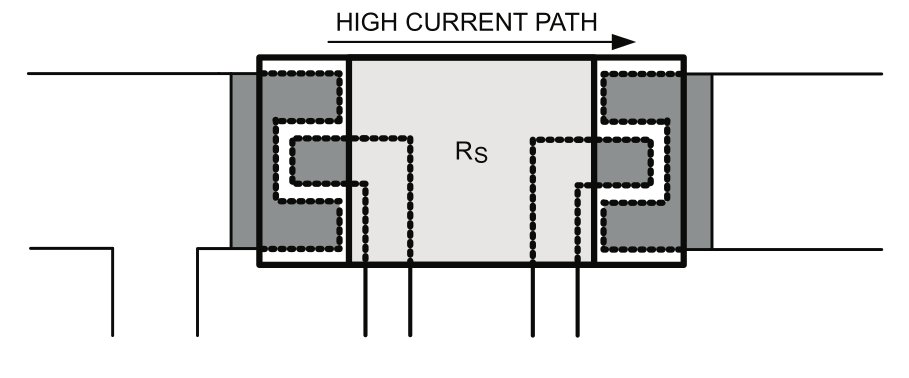
\includegraphics[scale=1.1]{Imagenes/Conexion Kelvin.png}
    \caption{Conexión Kelvin de cuatro cables para el sensado de corriente con un resistor shunt de montaje superficial.}
    \label{conexion_kelvin}
\end{figure}

Sin embargo, esto no puede solucionar el error introducido por el coeficiente de temperatura de las soldaduras, que se exacerban particularmente para valores bajos de resistencia. Para solventarlo, se debe utilizar la conexión de cuatro cables o Kelvin, que separa el camino de alta corriente de las conexiones de sensado, como se ve en la figura \ref{conexion_kelvin}.\textsuperscript{\cite{CurrentSensing}}\\

\subparagraph{Bobina de Rogowski}

Este es un método de medición de corriente basado en la Ley de Inducción de Faraday, y por lo tanto, {\Medium provee aislamiento eléctrico} por su propio principio funcionamiento, a diferencia del método anterior. Este dispositivo consiste, fundamentalmente, en una bobina de forma toroidal y núcleo no ferromagnético a través de la cual se hace pasar el conductor del que se quiere medir la corriente.\\

\begin{figure}[h]
    \centering
    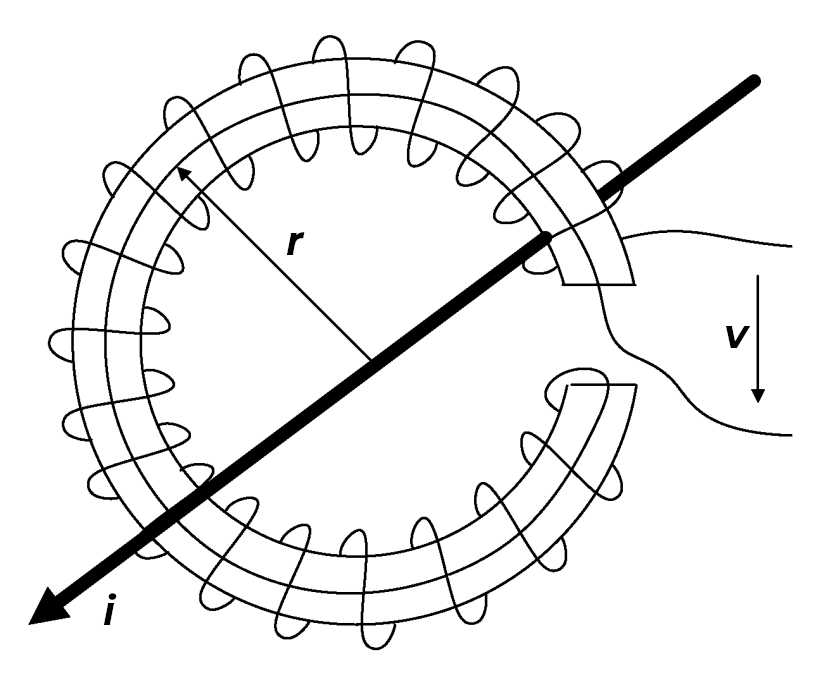
\includegraphics[scale=0.2]{Imagenes/Bobina Rogowski.png}
    \caption{Esquema de una bobina de Rogowski utilizada para medir la corriente $i$ que circula por el conductor.}
    \label{bobina_rogowski}
\end{figure}

Utilizando las leyes de Ampere (que relaciona la integral de un campo magnético en un camino cerrado con la corriente que este encierra) y Faraday (que relaciona la velocidad de cambio de un flujo magnético con la tensión o fuerza electromotriz) se puede obtener una expresión para la tensión medida en bornes de la bobina en función de la corriente de interés. Siguiendo el desarrollo de \cite{CurrentSensing}, se obtiene la siguiente expresión para la tensión de salida.

\begin{equation*}
    v = -\frac{NA\mu_0}{2\pi r}\cdot \frac{di}{dt}
\end{equation*}

Donde $N$ es la cantidad de vueltas de la bobina, $A$ es el área de un corte de la bobina, y $r$ es el radio de la bobina. Sin embargo, en esta ecuación la tensión de salida depende de la velocidad de cambio de la corriente que nos interesa. Entonces, se debe agregar un integrador de constante de integración $k$ a la salida de la bobina, para obtener la tensión $v_o$ dependiente de la corriente que nos interesa.

\begin{equation}\label{ec_rogowski}
    v_o = -k\cdot\frac{NA\mu_0}{2\pi r}\cdot i + v_o(0)
\end{equation}

Una gran ventaja de esta tecnología, es que al no utilizar un núcleo ferromagnético, tiene un rango de medición {\Medium altamente lineal}, comparable con el de una medición por shunt. Además de esto, al no tener que conectar nada al circuito en estudio, prácticamente {\Medium no introduce perturbaciones}, existiendo únicamente pequeños efectos causados por la inductancia de la bobina.\\

Comparado con el resistor shunt, este método presenta muy {\Medium bajas pérdidas} energéticas, al no tener circulación de altas corrientes. Por esta razón, este método es capaz de medir muy {\Medium grandes corrientes}, del orden de los \unit{\mega\ampere}, presentando una clara ventaja respecto al shunt.\\

Sin embargo, al estar su funcionamiento basado en la detección de un cambio de flujo magnético, este sensor es {\Medium incapaz de detectar corrientes continuas}, y tiene dificultades con la detección de componentes de baja frecuencia (es común la utilización de estas bobinas en conjunto con otros sensores capaces de detectar continua).\\

Otra desventaja que dificulta su implementación para nuestra aplicación, es que estas bobinas {\Medium ocupan un gran espacio} y no resulta sencillo integrarlas de forma compacta en una placa de circuito impreso. Además, por esto y por la necesidad de implementar un integrador, su costo es considerable frente al shunt.\\

\subparagraph{Transformador de Corriente}

Al igual que la bobina de Rogowski, este método se aprovecha de los principios establecidos por la ley de inducción de Faraday, por lo que también tiene {\Medium aislación intrínseca}. Su construcción es similar a las bobinas, con una vuelta de bobinado en el primario y una gran cantidad de vueltas en el secundario, pero a diferencia de estas, tiene un núcleo de material ferromagnético. Luego, conectada al secundario se encuentra una resistencia de sensado $R_S$ por la que circula la corriente de secundario $i_s$, generando una caída de tensión $v_s$. Se mide esta tensión, al igual que en el caso del shunt, y se obtiene la corriente del primario en función de esta.

\begin{equation*}
    i = Ni_s + \frac{N}{L_m}\int_t v_s\cdot dt
\end{equation*}

Donde $N$ es la cantidad de vueltas del transformador y $L_m$ es la inductancia magnetizante del transformador. Si reemplazamos la corriente del secundario $i_s$ por la expresión del shunt de la ecuación \ref{ec_shunt}, obtenemos la expresión de la corriente en función de la tensión medida.

\begin{equation}\label{ec_trafocorriente}
    i = N\frac{v_s}{R_S} + \frac{N}{L_m}\int_t v_s\cdot dt
\end{equation}

El término integral de esta ecuación indica que este método es {\Medium incapaz de medir corrientes continuas}: si la corriente $i$ del primario contiene componentes de CC, la corriente magnetizante aumenta hasta que todo el componente de corriente circula únicamente por la inductancia magnetizante $L_m$.\\

Como las vueltas $N$ del secundario pueden ser muy elevadas, se puede obtener una corriente de secundario muy baja, y en consecuencia unas {\Medium bajas pérdidas de energía}. Además, si el término integrador es pequeño (que es el caso para altas frecuencias), las corrientes de primario y secundario son prácticamente proporcionales, resultando en un sensor con {\Medium buena linealidad}.\\

\begin{figure}[h]
    \centering
    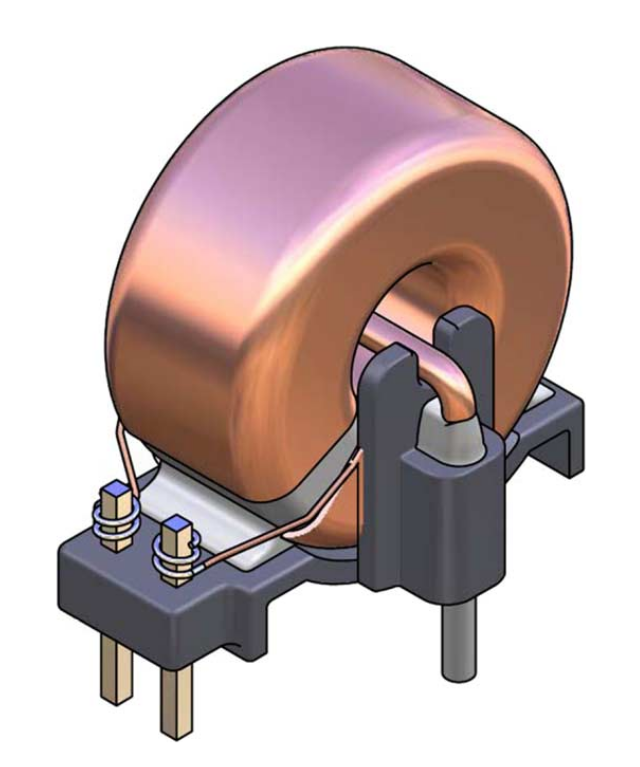
\includegraphics[scale=0.2]{Imagenes/Trafo Corriente.png}
    \caption{Transformador de corriente con una vuelta de primario y múltiples vueltas de secundario.}
    \label{trafo_corriente}
\end{figure}

La inductancia $L_m$ introduce errores de medición, ya que la corriente que circula por ella no circula por la resistencia de sensado, y por lo tanto esto disminuye la caída de tensión $v_s$. Este es un fenómeno conocido como \textit{droop}, y se exacerba particularmente para pulsos de corriente de tiempos largos de encendido en el primario (esto es de interés para nuestra aplicación, dados los pulsos generados por la conmutación de las llaves).\\

Además, como se ve en la figura \ref{trafo_corriente}, su integración en una plaqueta puede ser problemático por su {\Medium gran tamaño}. Sin embargo, hoy en día son muy populares en aplicaciones de convertidores, dado su {\Medium bajo costo} y su salida que suele ser directamente compatible con conversores analógico-digitales.\\

\subparagraph{Efecto Hall}

Finalmente, una tecnología que se utiliza mucho hoy en día son los sensores por efecto Hall, del tipo de medición de campo magnético, basados en el efecto homónimo descubierto por Edwin Hall en 1879. Este efecto consiste en una fina placa metálica sobre la que circula una corriente $I$, atravesada perpendicularmente por un campo magnético $B$, genera una diferencia de potencial $v$ perpendicular a ambos.

\begin{figure}[h]
    \centering
    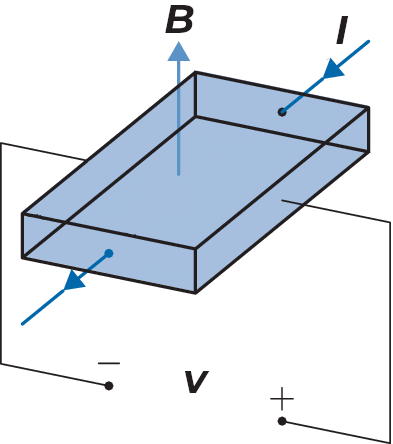
\includegraphics[scale=0.35]{Imagenes/Efecto Hall.png}
    \caption{Diagrama que muestra el principio de funcionamiento de un sensor de corriente por efecto Hall.}
    \label{efecto_hall}
\end{figure}

Entonces, generando un campo magnético que atraviese una placa por la que circula la corriente de interés $i$, se puede medir la tensión que cae en ellas y obtener por medio de esta el valor de la corriente según la ecuación de Hall.

\begin{equation}
    I = v\cdot\frac{nqd}{B}
\end{equation}

Dónde $q$ es la carga de los portadores, $n$ la densidad de portadores y $d$ el grosor de la placa. Como $n$ y $q$ son parámetros que dependen exclusivamente del material utilizado, se suelen consolidar en un parámetro llamado coeficiente de Hall $R_H$, que se define como la inversa del producto de $n$ y $q$. Entonces, la ecuación del sensor resulta:

\begin{equation}\label{ec_hall}
    I = v\cdot\frac{d}{R_HB}
\end{equation}

Como se puede ver por la ecuación, este método posee una {\Medium buena linealidad}, y además, como la corriente circula por un simple conductor, la perturbación introducida es mínima y tiene {\Medium bajas pérdidas de potencia}.\\

Al igual que los métodos de bobina de Rogowski y transformador de corriente, este método, por su principio de funcionamiento, ya {\Medium incluye aislación galvánica}. Pero, a diferencia de los otros métodos magnéticos e inductivos, los sensores de efecto Hall son perfectamente {\Medium capaces de realizar mediciones de corriente continua}.\\

En tanto a sus problemas, los materiales utilizados para las placas metálicas de los sensores suelen tener {\Medium elevadas constantes de temperatura}, por lo que pueden resultar muy susceptibles a cambios de temperatura por sobrecalentamiento. También, para un campo magnético nulo existe una tensión de salida de \textit{offset} no nula, por lo que se requiere electrónica adicional para compensar por este error.\\

Sin embargo, hoy en día existen soluciones integradas en pequeños empaquetados de montaje superficial como los SOIC o SOP, que incluyen un sensor de efecto hall con toda la electrónica asociada necesaria para compensar la tensión de offset y las variaciones por temperatura. Estas son soluciones compactas y de alta precisión, a pesar de su precio mayor comparado con otros métodos.\\\pagebreak

\subparagraph{Resumen}

A modo de resumen de todo lo explicado, se presenta la tabla \ref{tabla:resumen_sensores} que contiene las principales características de interés de las tecnologías de medición de corriente explicadas.\\

\setlength{\tabcolsep}{6pt}
\renewcommand{\arraystretch}{1.5}
\begin{table}[h]
\begin{center}
    \begin{tabular}{llllll}
        & {\SemiBold Ancho de Banda} & {\SemiBold Precisión} & \makecell[l]{{\SemiBold Medición} \\ {\SemiBold de CC}} & {\SemiBold Aislación} & {\SemiBold Pérdidas}\\
        \hline
        Shunt & \unit{\kilo\hertz}-\unit{\mega\hertz} & \num{0,1}\% - \num{2}\% & Sí & No & \unit{\milli\watt}-\unit{\watt}\\
        \makecell[l]{Bobina de \\ Rogowski} & \unit{\kilo\hertz}-\unit{\mega\hertz} & \num{0,1}\% - \num{1}\% & No & Sí & \unit{\milli\watt}\\
        Transformador & \unit{\kilo\hertz}-\unit{\mega\hertz} & \num{0,1}\% - \num{1}\% & No & Sí & \unit{\milli\watt}\\
        Efecto Hall & \unit{\kilo\hertz} & \num{0.5}\% - \num{5}\% & Sí & Sí & \unit{\milli\watt}
    \end{tabular}
    \caption{Resumen de las características principales de cada tecnología de sensado de corriente.\textsuperscript{\cite{CurrentSensing}}}
    \label{tabla:resumen_sensores}
\end{center}
\end{table}

Con la información de los distintos tipos de sensores de corriente que se explicaron, se deben seleccionar los modelos de los sensores de la tecnología adecuada para la medición de las variables, buscando en catálogos de sensores.\\

\paragraph{Sensor de Corriente $\mathbf{i_o}$}

La corriente de salida $i_o$ es la variable a medir más importante, ya que es la que directamente controla la potencia de salida que se entrega al bus de continua del sistema híbrido. Por esta razón, debe cumplir algunos requerimientos que se enumeran a continuación.\\

\begin{itemize}
    \item Capacidad de corriente mayor a \SI[]{4.5}[]{\ampere}.
    \item Tensión de operación mayor a \SI[]{100}[]{\volt}.
    \item Precisión de medición debajo del $\pm$1\%.
    \item Ancho de banda $BW$ por encima de \SI[]{40}[]{\kilo\hertz}, el doble de la frecuencia de conmutación.
    \item Capacidad de medir componentes de CC.
    \item Es deseable que el sensor esté galvánicamente aislado del circuito del convertidor.\\
\end{itemize}

La necesidad de medir componentes de corriente continua elimina automáticamente la posibilidad de usar una bobina de Rogowski o un transformador de corriente. Por lo tanto, nos quedan como opciones únicamente la resistencia shunt y el sensor de efecto Hall, que dado que ambos son capaces de precisiones debajo del \num{1}\% y anchos de banda de \unit{\kilo\hertz}, se decide utilizar un {\Medium sensor de efecto Hall}, por la presencia de aislación galvánica.\\

Entonces, buscando sensores de corriente de efecto Hall en catálogos online, se llegó al modelo {\Medium TMCS1100A4} de Texas Instruments, un sensor Hall de medición bidireccional (corrientes positivas y negativas) de alta precisión y aislamiento básico, todo en un encapsulado de montaje superficial de ocho pines tipo SOIC-8. Según la hoja de datos del fabricante, este dispostivo esta pensado para ser utilizado en la medición de corrientes de inversores y puentes completos. Sus especificaciones se presentan en la tabla \ref{tabla:sensor_hall}.\\

\setlength{\tabcolsep}{6pt}
\renewcommand{\arraystretch}{1.5}
\begin{table}[H]
\begin{center}
    \begin{tabular}{llrrrrr}
    {\SemiBold Fabricante} & {\SemiBold Modelo} & $\mathbf{I_{in}}$ [\unit{\ampere}] & $\mathbf{V_{in}}$ [\unit{\volt}] & $\mathbf{BW}$ [\unit{\kilo\hertz}] & $\mathbf{e_i}$ & {\SemiBold Sens.} [\unit{\milli\volt\per\ampere}]\\
    \hline
    \makecell[l]{Texas \\ Instruments} & TMCS1100A4 & \num{12} & \num{600} &  \num{80} & $\pm$\num{0.9}\% & \num{400}
    \end{tabular}
    \caption{Especificaciones del sensor de corriente por efecto Hall, modelo TMCS1100A4 de Texas Instruments.\textsuperscript{\cite{TMCS1100}}}
    \label{tabla:sensor_hall}
\end{center}
\end{table}

Dónde $I_{in}$ es la máxima corriente unidireccional medible, $V_{in}$ es la máxima tensión de operación en la entrada, $BW$ es el ancho de banda de la medición, y $e_i$ es la precisión o error relativo de la medición.\\ 

La variante A4 tiene una sensibilidad de \SI[]{400}[]{\milli\volt\per\ampere}, poniendo la tensión de salida en el rango de \num{0} a \SI[]{1.8}[]{\volt} para una corriente de salida $i_o$ máxima de \SI[]{4.5}[]{\ampere}. Además, si tomamos el error relativo máximo de $\pm$\num{0.9}\%, se obtiene que la precisión absoluta es de $\pm$\SI[]{40}[]{\milli\ampere}, más que suficiente para ser aplicado en la plataforma.\\

\begin{figure}[h]
    \centering
    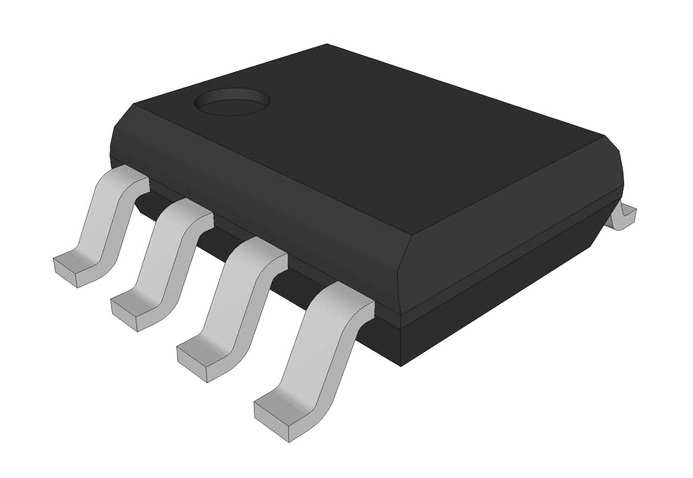
\includegraphics[scale=0.8]{Imagenes/SOIC8.jpg}
    \caption{Sensor de corriente por efecto Hall, modelo TMCS1100A4 de Texas Instruments, en su encapsulado tipo SOIC-8.}
    \label{encapsulado_hall}
\end{figure}

El sensor tiene cuatro pines para el sensado de corriente, dos llamados IN+ y dos llamados IN-. Como se trata de medición de corriente, se debe conectar el sensor en serie al camino de corriente, con la corriente entrando por los pines IN+ y saliendo por los pines IN-.\\

Luego, el pin de tensión de referencia VREF se conecta a masa, que de esta manera configura el sensor para utilizar un rango de medición unidireccional (configurando la tensión de salida nula para corriente nula)\textsuperscript{\cite{TMCS1100}}, ya que en nuestro caso la corriente solo puede circular hacia la carga.\\

\begin{figure}[h]
    \centering
    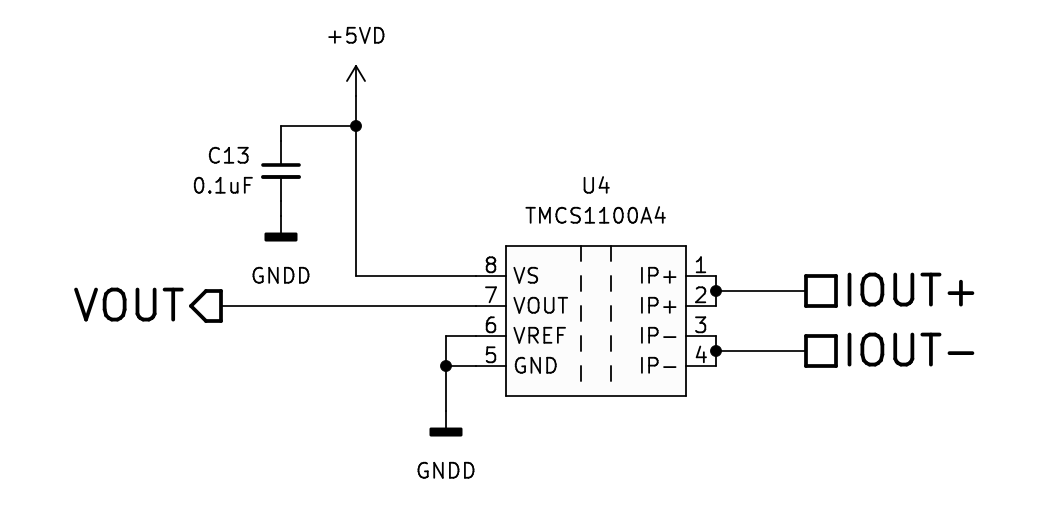
\includegraphics[scale=1]{Imagenes/Conexion TMCS1100.png}
    \caption{Conexión del sensor TMCS1100A4, según recomendaciones del fabricante.}
    \label{conexion_TMCS1100}
\end{figure}

Todas las conexiones a tierra del sensor se realizan en la tierra de señal o digital $GND_D$, ya que se encuentran todas del segundo lado del dispositivo, aislados del circuito de potencia del convertidor. El pin VS se conecta a la alimentación digital del sistema requiriendo una tensión de \SI[]{5}[]{\volt} positivos, con un capacitor de filtro conectado en derivación según recomendación del fabricante.\\

El pin de salida VOUT, como se verá mas adelante, se debe conectar primero a un circuito que acondicione la señal que el sensor arroja, para luego poder ser conectado a la entrada del conversor analógico-digital (ADC) del controlador que convertirá los datos analógicos de corriente en datos digitales que pueda procesar.\\

\paragraph{Sensor de $\mathbf{v_{FC}}$, $\mathbf{i_{FC}}$ y $\mathbf{v_o}$}

Por una cuestión de simplicidad, se eligió buscar una única solución integrada que sea capaz de medir múltiples variables, en nuestro caso una corriente y dos tensiones. Dado que las variables restantes son de menor importancia, limitar el requerimiento de ancho de banda respecto a la corriente de salida. A continuación se detallan algunos requerimientos.\\

\begin{itemize}
    \item Capacidad de medición de corriente por arriba de \SI[]{11}[]{\ampere}.
    \item Capacidad de medición de tensión por arriba de \SI[]{75}[]{\volt}.
    \item Precisión mejor o igual al $\pm$\num{2}\%.
    \item Capacidad de medir componentes de CC.
    \item Ancho de banda $BW$ lo más alto posible.
    \item Es deseable que el sensor esté galvánicamente aislado del circuito del convertidor.\\
\end{itemize}

Buscando en catálogos online de distintos fabricantes se encontró el {\Medium circuito integrado LM5056A} de Texas Instruments, descrito por el fabricante como un \quotes{Dispositivo de Administración de Potencia de Sistemas de Alta Tensión}.\\

Consiste en un sensor de corriente de tipo shunt, junto con un sensor de tensión a la entrada del shunt y una medición de tensión secundaria, con la capacidad adicional de calcular la potencia en base a las mediciones.  Al usar medición de tipo shunt, tiene la capacidad de medir componentes de CC, pero no posee aislación galvánica. Se detallan algunas especificaciones a continuación.\\

\setlength{\tabcolsep}{6pt}
\renewcommand{\arraystretch}{1.5}
\begin{table}[H]
\begin{center}
    \begin{tabular}{llrrrrr}
    {\SemiBold Fabricante} & {\SemiBold Modelo} & $\mathbf{V_{in/out}}$ [\unit{\volt}] & $\mathbf{f_m}$ [\unit{\kilo\hertz}] & $\mathbf{I_{in(FSR)}}$ [\unit{\milli\volt}] & $\mathbf{e_{i}}$ & $\mathbf{e_v}$\\
    \hline
    \makecell[l]{Texas \\ Instruments} & LM5056A & \num{100} & \num{1} &  \num{27}/\num{54.4} & $\pm$\num{1.25}\% & $\pm$\num{1}\%
    \end{tabular}
    \caption{Especificaciones del sensor combinado de tensión, corriente y potencia por shunt, modelo LM5056A de Texas Instruments.\textsuperscript{\cite{LM5056A}}}
    \label{tabla:LM5056A}
\end{center}
\end{table}

Donde $V_{in/out}$ es la máxima tensión de entrada y salida medible, $f_m$ es la frecuencia de muestreo del sensor, $I_{in(FSR)}$ es la tensión de fondo de escala de medición de corriente, $e_i$ es la precisión de la medida de corriente, y $e_v$ es la precisión de la medida de tensión.\\

Los parámetros analógicos de tensión y corriente medidos por el LM5056A son muestreados y convertidos a información digital mediante un conversor analógico-digital interno de \num{12} bits de resolución, (es decir $2^{12} = 4096$ niveles distintos) con frecuencia de muestreo $f_m$ de \SI[]{1}[]{\kilo\hertz} como muestra la tabla. Una vez convertidos, se pueden transmitir mediante la interfaz de bus I\textsuperscript{2}C que provee el integrado, con pines SDAO para salida de datos, SDAI para entrada de datos y SCL para entrada de reloj. Esta interfaz se explica más adelante en la sección 3.4.3, sobre la etapa de transmisión.\\

Este dispositivo viene en un empaquetado de montaje superficial del tipo HTSSOP-28 de veintiocho pines (figura \ref{encapsulado_LM5056}), que también incluye un contacto plano en la parte inferior, de conexión opcional para la disipación de calor.\\

\begin{figure}[h]
    \centering
    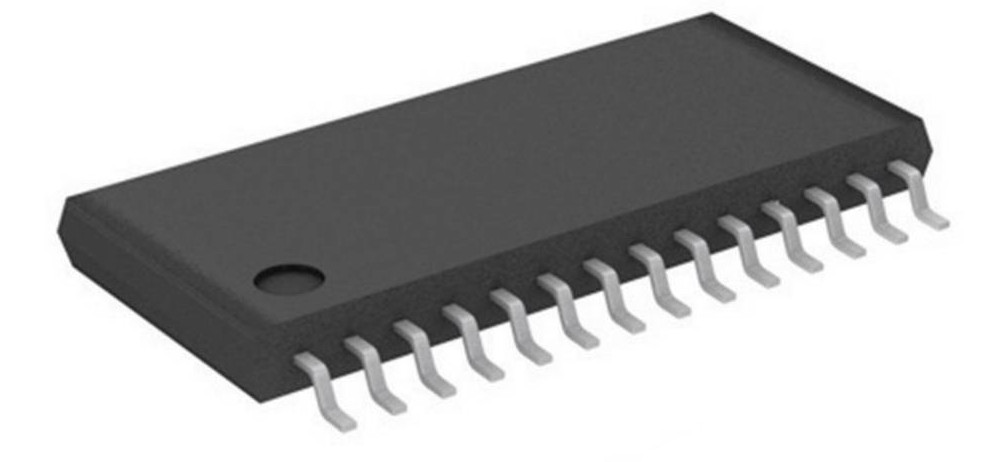
\includegraphics[scale=0.15]{Imagenes/HTSSOP.jpg}
    \caption{Sensor de tensión, corriente y potencia, modelo LM5056A de Texas Instruments, en su encapsulado tipo HTSSOP-28.}
    \label{encapsulado_LM5056}
\end{figure}

Además de lo ya mencionado, el LM5056A tiene un pin al que se puede conectar un circuito que permite la medición de temperatura mediante la utilización de un transistor NPN modelo MMBT3904 conectado al pin DIODE, y medición de una tensión auxiliar de bajo valor mediante el pin VAUX.\\

En la figura \ref{conexion_LM5056A}, se puede ver el esquema circuital del LM5056A dentro de la plataforma de evaluación. Los pines de medición principales son OUT, SENSE, VIN\_K y VIN. Al pin OUT se conecta la tensión de medición secundaria, que en nuestro caso es la tensión de carga $v_o$ fija de \SI[]{75}[]{\volt}. Luego, entre VIN\_K y SENSE se conecta la resistencia shunt $R_{shunt}$ para la medición de la corriente $i_{FC}$ de máximo de \SI[]{10.5}[]{\ampere}, con un capacitor $C_{shunt}$ de \textit{bypass} en paralelo a $R_{shunt}$ según indicación del fabricante. Finalmente, el pin VIN se conecta al mismo punto circuital que VIN\_K, para poder medir la tensión de celda $v_{FC}$, variable entre \SI[]{30}[]{\volt} y \SI[]{65}[]{\volt}, con un capacitor de bypass para mejorar rendimiento en situaciones ruidosas, según recomendacion de fabricante.\\

\begin{figure}[h]
    \centering
    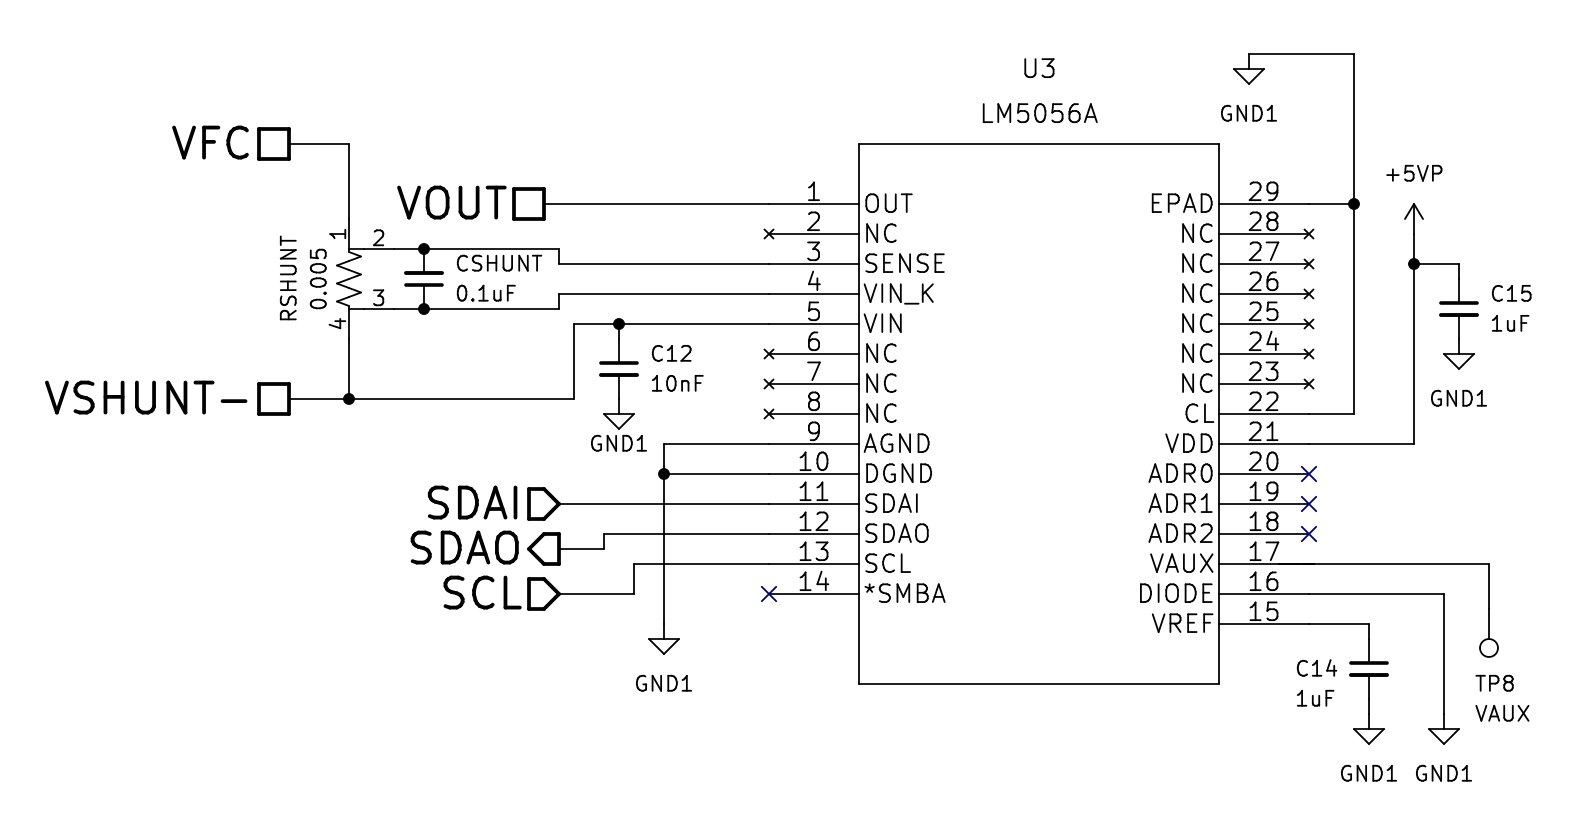
\includegraphics[scale=0.22]{Imagenes/Conexion LM5056A.png}
    \caption{Conexión del sensor LM5056A para medir tensión y corriente de entrada y tensión de salida, según especificaciones del fabricante.}
    \label{conexion_LM5056A}
\end{figure}

Como el dispositivo no tiene aislación incluida, todas sus tierras se conectan al punto común del primario del convertidor, $GND_1$. Luego, el pin CL se utiliza para la selección de rango de medición para la corriente, que puesto a tierra como en la figura, resulta en un fondo de escala de \SI[]{54.4}[]{\milli\volt}. El pin VAUX se deja abierto en caso de ser necesario la medición de una tensión auxiliar, DIODE se deja conectado a masa ya que no se necesita una medición de temperatura. Según el fabricante, al pin VREF se debe conectar un capacitor de bypass desde este pin a $GND_1$. La alimentación del LM5056A, conectado al pin VDD, es de \SI[]{5}[]{\volt}, con un capacitor de bypass en derivación entre alimentación y tierra.\\

Finalmente, para calcular el valor que debe tener el resistor shunt $R_{shunt}$ se toma en cuenta el valor máximo de corriente a medir $i_{FC}$ con algún margen de seguridad, que en nuestro caso es \SI[]{11}[]{\ampere}. Después, utilizando la tensión de fondo de escala de \SI[]{54.4}[]{\milli\volt} elegida para la medición de corriente, se puede obtener el valor de $R_{shunt}$ realizando el cociente entre tensión y corriente, que resulta en un valor de shunt de \SI[]{5}[]{\milli\ohm}.

\begin{equation}\label{calculo_shunt}
    \boxed{\highlight{
    R_{shunt} = \frac{I_{in(FSR)}}{i_{FC(max)}} = \frac{\SI{54.4}{\milli\volt}}{\SI{11}{\ampere}} \approx \SI[]{5}[]{\milli\ohm}
    }}
\end{equation}

\subsubsection{Etapa de Acondicionamiento}

Una vez seleccionados los sensores, muchas veces es necesario agregar a la salida de los mismos un circuito de acondicionamiento, cuyo objetivo es adecuar los niveles de tensión y/o corriente que provee la salida del sensor a los niveles que son requeridos en la entrada de la siguiente etapa. En nuestro caso, esta etapa siguiente es el sistema de control de la plataforma, cuyo diseño se va a profundizar más adelante.\\

Para el sensor LM5056A de la figura \ref{conexion_LM5056A} no es necesario implementar ninguna etapa de acondicionamiento, ya que el mismo transmite sus datos a través de su módulo de comunicación sincrónica $I^2C$, actuando como esclavo y el controlador como maestro. Esta dinámica se explica en detalle en la siguiente sección.\\

\paragraph{Acondicionamiento de $\mathbf{i_o}$}

El sensor de corriente de salida TMCS1100A4 de la figura \ref{conexion_TMCS1100} tiene una salida de tensión analógica, variable linealmente entre \SI[]{0}[]{\volt} y \SI[]{1.8}[]{\volt} para corriente $i_o$ desde nula hasta \SI[]{4.5}[]{\ampere}. Esta señal debe ingresar al conversor analógico-digital de \num{12} bits y \num{4096} niveles del DSC, que toma tensiones de entrada desde \SI[]{0}[]{\volt} hasta \SI[]{3}[]{\volt}.\\

Entonces, como tanto la salida del sensor y la entrada de ADC tienen su origen en tensión nula y solo difieren en la máxima tensión que aceptan, se debe diseñar un circuito de acondicionamiento con una {\Medium ganancia positiva} que lleve los \SI[]{1.8}[]{\volt} del sensor al fondo de escala del ADC, de manera de aprovechar la resolución completa del conversor. Entonces, la ganancia $G_{cc}$ que debemos obtener del circuito se puede obtener con el cociente de las tensiones máximas.

\begin{equation}\label{ganancia_acond}
    G_{cc} = \frac{V_{max(ADC)}}{V_{max(Sensor)}} = \frac{\SI{3}{\volt}}{\SI{1.8}{\volt}} \approx 1.67
\end{equation}

Y como ambas escalas comienzan en cero, no es necesario que el circuito tenga ningún tipo de tensión de offset. Además, la salida del sensor y entrada al ADC del controlador son señales {\Medium \textit{single-ended}} (es decir que solo tiene un conductor para la señal y otro para la tensión de referencia de tierra), por lo que solo es relevante la amplificación single-ended del circuito.\\

Para este propósito, se eligió un {\Medium amplificador diferencial} basado en un amplificador operacional, con una red de resistencias y capacitores que definen su ganancia $A_d$ y ancho de banda $BW$, que observa en la figura \ref{circuito_acond}. Este circuito, además de proveer la adaptación de niveles, actúa como un filtro pasabajos que le da al sistema una mayor inmunidad al ruido.\\

\begin{figure}[h]
    \centering
    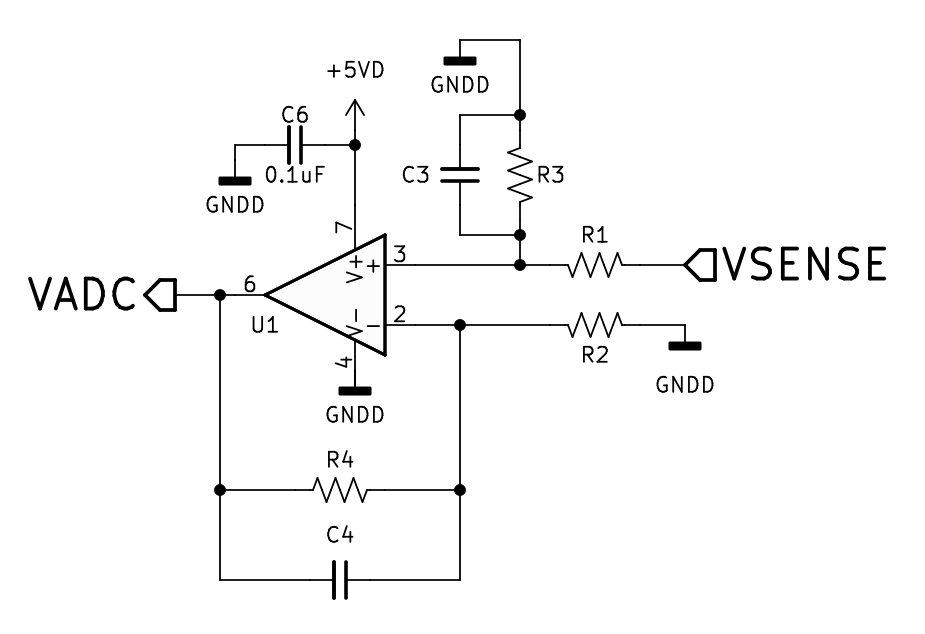
\includegraphics[scale=1.2]{Imagenes/Acondicionamiento.png}
    \caption{Circuito del amplificador diferencial de acondicionamiento, utilizando un amplificador operacional.}
    \label{circuito_acond}
\end{figure}

Como el amplificador es diferencial pero la tensión a la entrada es single-ended ,y no se busca un amplificador inversor, se conecta la tensión de salida del sensor al pin positivo de entrada del operacional, con el pin negativo conectado a tierra. En este amplificador, se deben cumplir un par de condiciones, particularmente, las resistencias $R_1$ y $R_2$ deben ser iguales, al igual que las impedancias $Z_3$ y $Z_4$, que resultan del paralelo de las resistencias y las impedancias de los capacitores $C_3$ y $C_4$ a la frecuencia $f_s$ de interés de \SI[]{20}[]{\kilo\hertz}.\\

Con estas condiciones, y asumiendo las características de un amplificador operacional ideal (tensiones $v_+$ y $v_-$ idénticas, y corrientes $i_+$ e $i_-$ nulas), se obtienen las siguientes dos expresiones para la ganancia y el ancho de banda del circuito.\textsuperscript{\cite{Caravelli-Irusta}\cite{DifferenceAmps}}\\

\begin{equation}\label{ec_gcc}
    G_{cc} = \frac{Z_3}{R_1} = \frac{Z_4}{R_2}
\end{equation}

\begin{equation}\label{ec_bw}
    BW = \frac{1}{2\pi R_3C_3} = \frac{1}{2\pi R_4C_4}
\end{equation}

Entonces, si tomamos como requerimientos la ganancia $G_{cc}$ de \num{1.67} de la ecuación \ref{ganancia_acond} y un ancho de banda $BW$ (frecuencia de \SI[]{-3}[]{\deci\bel}) de \SI[]{100}[]{\kilo\hertz} mucho mayor a la frecuencia de conmutación del convertidor, y elegimos (arbitrariamente) resistencias $R_1$ y $R_2$ de \SI[]{16.5}[]{\kilo\ohm}, podemos despejar entonces la impedancia $Z_3$ de la ecuación \ref{ec_gcc}.

\begin{equation}
    Z_3 = Z_4 = G_{cc}R_1 = \SI{27.55}{\kilo\ohm}
\end{equation}

Con este valor y los requerimientos más arriba, tenemos que calcular los valores de ambos componentes del paralelo de $Z_3$ (o $Z_4$), $R_3$ y $C_3$ (o $R_4$ y $C_4$). Con este objetivo, planteamos la ecuación este paralelo.

\begin{equation}
    Z_3 = \frac{R_3\cdot X_{C3}}{R_3+X_{C3}} = \SI{27.55}{\kilo\ohm}
\end{equation}

Donde $X_{C3}$ es la impedancia capacitiva del paralelo, definido como el inverso del producto de la frecuencia angular de interés por la capacidad del capacitor $C_3$. Reemplazando por esta expresión, obtenemos la siguiente ecuación.

\begin{equation}\label{eq_z3}
        Z_3 = \frac{R_3}{2\pi fC_3R_3 + 1} = \SI[]{27.55}[]{\kilo\ohm}
\end{equation}

Con esta ecuación y la ecuación \ref{ec_bw} del ancho de banda de la topología, podemos conformar un sistema de ecuaciones de dos variables y dos ecuaciones no lineales.

\begin{equation}\label{sist_eq}
    \begin{aligned}
        \frac{R_3}{2\pi fC_3R_3 + 1} &= \SI[]{27.55}[]{\kilo\ohm}\\
        \frac{1}{2\pi R_3C_3}        &= \SI[]{100}[]{\kilo\hertz}
    \end{aligned}
\end{equation}

Entonces, si despejamos $R_3$ y $C_3$ de este sistema de ecuaciones, obtenemos los siguientes valores para los mismos (recordar que $R_4$ y $C_4$ deben ser idénticos).

\begin{equation*}
    \begin{aligned}
        R_3 = R_4 &= \SI[]{33.06}[]{\kilo\ohm}\\
        C_3 = C_4 &= \SI[]{48.1}[]{\pico\farad}
    \end{aligned}
\end{equation*}

Ahora solo falta redondear estos parámetros a los valores comerciales más cercanos para cada uno de los componentes, que se observan en la siguiente tabla.\\

\setlength{\tabcolsep}{8pt}
\renewcommand{\arraystretch}{1.5}
\begin{table}[H]
\begin{center}
    \begin{tabular}{rrrrrr}
    $\mathbf{R_1}$ [\unit{\kilo\ohm}] & $\mathbf{R_2}$ [\unit{\kilo\ohm}] & $\mathbf{R_3}$ [\unit{\kilo\ohm}] & $\mathbf{R_4}$ [\unit{\kilo\ohm}] & $\mathbf{C_3}$ [\unit{\pico\farad}] & $\mathbf{C_4}$ [\unit{\pico\farad}]\\
    \hline
    \num{16.5} & \num{16.5} & \num{33} & \num{33} & \num{47} & \num{47}
    \end{tabular}
    \caption{Valores comerciales de todas las resistencias y capacitores del circuito de acondicionamiento.}
    \label{tabla:componentes_acond}
\end{center}
\end{table}

Si usamos estos valores finales para calcular las especificaciones de las ecuaciones de ganancia y ancho de banda, se obtienen los siguientes valores:

\begin{equation*}
    \boxed{\highlight{
    \begin{aligned}
        G_{cc} &= \num{1.673}\\
        BW &= \SI[]{102.6}[]{\kilo\hertz}
    \end{aligned}
    }}
\end{equation*}

\paragraph{Selección del Amplificador Operacional}

Con el circuito de acondicionamiento diseñado y dimensionado ahora solo queda la elección de un amplificador operacional para utilizar en el circuito, que cumpla los siguientes requerimientos.\\

\begin{itemize}
    \item Debe ser un amplificador \textit{rail-to-rail}, es decir que sea capaz de amplificar hasta la tensión de alimentación.
    \item Ancho de banda mucho mayor a \SI[]{100}[]{\kilo\hertz}.
    \item Encapsulado pequeño de montaje superficial.\\
\end{itemize}

Buscando en los dispositivos disponibles en el laboratorio, se eligió utilizar el modelo {\Medium OPA365} de Texas Instruments, un amplificador operacional rail-to-rail de encapsulado SMD tipo SOIC-8, idéntico al del sesnor TMCS1100A4 de la figura \ref{encapsulado_hall}. Se marcaron algunas de sus especificaciones más importantes en la siguiente tabla.\\

\setlength{\tabcolsep}{7pt}
\renewcommand{\arraystretch}{1.5}
\begin{table}[H]
\begin{center}
    \begin{tabular}{llrrrr}
    {\SemiBold Fabricante} & {\SemiBold Modelo} & $\mathbf{V_{in(max)}}$ [\unit{\volt}] & $\mathbf{V_{DD(max)}}$ [\unit{\volt}] & $\mathbf{A_{OL}}$ [\unit{\deci\bel}] & $\mathbf{GBW}$ [\unit{\mega\hertz}]\\
    \hline
    Texas Instruments & OPA365 & $V_{DD}$ + \num{0.5} & \num{5.5} &  \num{120} & \num{50}
    \end{tabular}
    \caption{Especificaciones del amplificador operacional modelo OPA365 de Texas Instruments.\textsuperscript{\cite{OPA365}}}
    \label{tabla:OPA365}
\end{center}
\end{table}

Al ubicarse el circuito de acondicionamiento a continuación de la salida del sensor de efecto Hall TMCS1100A4 (que provee su propia aislación galvánica), las conexiones a tierra de todas las partes deben ser conectadas a la tierra digital o de señal $GND_D$.\\

\subsubsection{Etapa de Transmisión}

Para transmitir los datos de tensión y corriente de entrada, y tensión de salida que entrega el monitor de potencia LM5056A, se utiliza, como se mencionó brevemente, el protocolo de transmisión de datos en serie I\textsuperscript{2}C o bus I\textsuperscript{2}C, ya que el sensor ya incluye internamente un controlador y firmware que se encarga de transmitir los datos obtenidos por este bus.\\

\paragraph{Bus I\textsuperscript{2}C}

Este protocolo, diseñado por Phillips Semiconductor (hoy en día NXP Semiconductor) en 1982, es un protocolo multi-dispositivo, sincrónico, de dos líneas, de esquema maestro/esclavo, de paquete conmutado o \textit{packet-switched}, single-ended, y de tipo half-duplex, principalmente utilizado para comunicación con componentes dentro de la plaqueta.\\

\begin{figure}[h]
    \centering
    
\includegraphics[scale=0.9]{Imagenes/Logo I2C.pdf}
    \caption{Logotipo del protocolo de transmisión de datos en serie I\textsuperscript{2}C.}
    \label{logo_I2C}
\end{figure}

\begin{itemize}
    \item {\Medium Multi-dispositivo:} El bus I\textsuperscript{2}C tiene la capacidad de transmitir datos entre múltiples dispositivos.
    \item {\Medium Sincrónico:} La transmisión de datos entre los dispositivos conectados al bus es sincronizada mediante una señal de reloj.
    \item {\Medium Dos líneas:} El bus solo cuenta con dos líneas para transmitir datos: la línea de datos bidireccional SDA y la línea de señal de reloj para sincronización SCL.
    \item {\Medium Maestro-esclavo:} En el protocolo se define uno o varios dispositivos maestros que generan la señal de reloj e inician la comunicación con los esclavos, y uno o varios dispositivos esclavos que reciben la señal de reloj y responden cuando el maestro lo indica.
    \item {\Medium Packet-switched:} El protocolo indica que los datos son transmitidos en \textit{paquetes} que cuentan con dos partes: los datos o \textit{payload}, y la información de control o \textit{header}.
    \item {\Medium Single-ended:} La señalización de los datos está referenciada a tierra, a diferencia de la señalización diferencial.
    \item {\Medium Half-duplex:} El bus no permite la transmisión de datos en ambas direcciones simultáneamente, ya que posee una única linea de datos bidireccional.\\
\end{itemize}

Otra característica importante del bus I\textsuperscript{2}C que lo diferencia de otros protocolos de comunicación serie es la utilización de {\Medium líneas de tipo \textit{open-drain}}: al transmitir datos o la señal de reloj, los dispositivos pueden bajar la línea a una tensión (generalmente tierra) para indicar un 0 lógico, o bien \quotes{soltar} la línea para que una resistencia de pull-up $R_{PU}$ levante la línea a la tensión de alimentación, indicando un 1 lógico.\\

\begin{figure}[h]
    \centering
    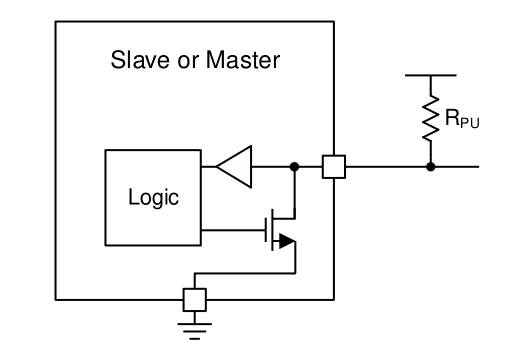
\includegraphics[scale=0.3]{Imagenes/Diagrama Open-Drain.png}
    \caption{Diagrama que muestra un dispositivo conectado a una línea I\textsuperscript{2}C con una resistencia de pull-up, exponiendo el funcionamiento del open-drain.\textuperscript{\cite{I2C}}}
    \label{opendrain_i2c}
\end{figure}

En la figura \ref{opendrain_i2c}, cuando el dispositivo quiere indicar un 0 activa el transistor, conectando la línea directamente con tierra; mientras que al indicar un 1, el transistor interno se desactiva y la línea queda flotante, siendo levantada a la tensión de alimentación por $R_{PU}$.\\

Con esta topología, si un dispositivo quiere transmitir un nivel bajo y otro dispositivo quiere transmitir un nivel alto no se genera ningún conflicto de comunicación, ya que los dispositivos no tienen la capacidad de forzar un nivel alto. Si este no fuese el caso, al forzar un alto cuando un dispositivo transmite un bajo se formaría un corto entre alimentación y tierra. Esta funcinalidad es la que le permite al bus implementar comunicación bidireccional.\textsuperscript{\cite{I2C}}\\

\subparagraph{Operación del Bus}



